% !TEX TS-program = pdflatex

\documentclass[unicode,11pt,notheorems]{beamer}

\usepackage[T2A]{fontenc}
\usepackage[utf8]{inputenc}
\usepackage[russian]{babel}
\usepackage{amsmath,amsfonts,amssymb,amsthm}
\usepackage{mathtools}

\usepackage{xcolor,colortbl,tabularx,array}
\usepackage{ulem}
\usepackage{tikz, graphicx}
%\usepackage{tkz-graph}
\usetikzlibrary{matrix,arrows,decorations.pathmorphing, arrows.meta,positioning}
\usetikzlibrary{positioning,calc}
\usetikzlibrary{petri}
\usetikzlibrary{decorations.pathreplacing}

%Описание стиля презентации
\usetheme[sidebar=0]{kfmn} 
\setbeamercovered{transparent}

%\definecolor{cyan}{RGB}{240,217,1}
%\definecolor{vgugreen}{RGB}{143,188,103}
%\definecolor{vgured}{RGB}{234,38,40}
%\definecolor{vgublue}{RGB}{53,101,167}

\newcommand{\myunit}{9mm}
\tikzset{
    node style sp/.style={draw,circle,minimum size=\myunit},
    node style ge/.style={circle,minimum size=\myunit},
    arrow style mul/.style={draw,sloped,midway,fill=white},
    arrow style plus/.style={midway,sloped,fill=white},
}

%[0, 6, 8, 8, 10, 5, 6, 10, 8, 10, 10], 

\pgfdeclareimage[height=8mm]{university-logo}{logo-iem.png}
\logo{\pgfuseimage{university-logo}}
%2[0, 11, 10, 8, 11, 5, 11, 11, 8, 11, 10, 11],

\titlepicture{
	\begin{tikzpicture}[y=1.4cm,overlay,rotate=8]
	\coordinate (O) at (-3cm,0.9cm);
	\filldraw[thick,draw= vgublue, fill=vgublue!20!white] (0,0) circle[radius=4.2cm];
	\clip (0,0) circle[radius=4.2cm];
	\draw (-1.5,1.5) node{
	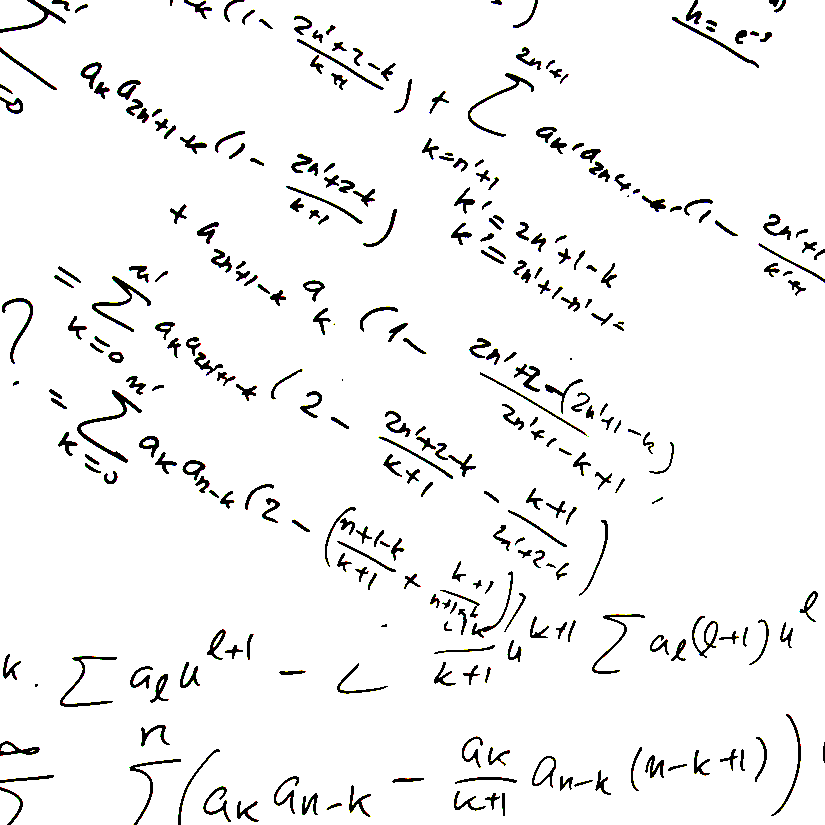
\includegraphics[width=8cm]{titlepic.png}
	};
\end{tikzpicture}
}

\usepackage[math]{iwona}

\newcommand{\hplus}{\mathbin{\hat+}}
\newcommand{\hdot}{\mathbin{\hat\cdot}}
% Описание теорем
\newtheorem{theorem}{Теорема}
\newtheorem{seq}{Следствие}
%%

%\VKR
\LECT % можно ещё лекцию забацать.
%\REPORT % можно ещё лекцию забацать.

%\titlepicture{
%%	\begin{tikzpicture}[overlay]
%%			\draw[opacity=0.4]  (-0.3,1.8) node {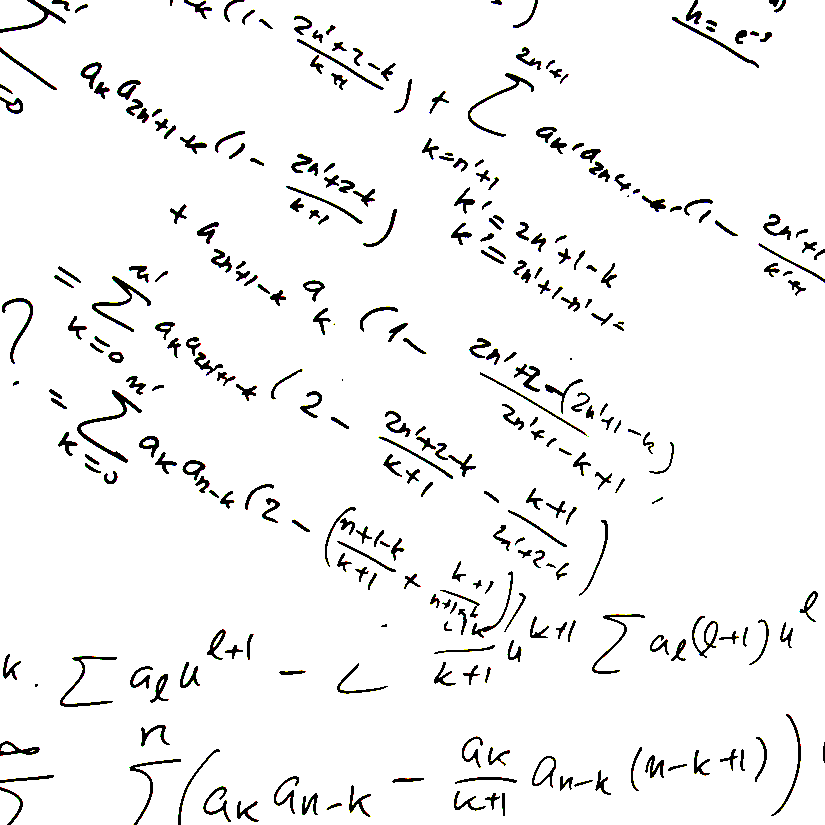
\includegraphics[width=3.5cm]{titlepic.png}};
%%	\end{tikzpicture}
%}

% Титульный лист теорем
\author[Д.\,В. Чупраков]{канд.\,физ.-матем.\,наук, доцент Д.\,В. Чупраков\\[6pt] usr10381@vyatsu.ru}

\institute[ВятГУ]{ФГБОУ ВО Вятский государственный университет}

\department{Факультет экономики и финансов}

\title[Лекция~4. Линейные задачи. Часть~2 из 4]{
	Введение в экономико-математическое моделирование\\[12pt]
	Лекция 4. Линейные задачи--2}
\subtitle{Исследование систем линейных уравнений. Метод Гаусса. Системы линейных неравенств}


\date{22 cентября 2020 г.}


%\setbeamercolor{coloredboxstuff}{fg=yellow,bg=white!10!blue}

\setbeamercovered{invisible}


\tikzset{
	 myarrow/.style={->, >=latex', shorten >=1pt, thick}
}



\tikzset{add/.style n args={4}{
    minimum width=6mm,
    path picture={
        \draw[black] 
            (path picture bounding box.south east) -- (path picture bounding box.north west)
            (path picture bounding box.south west) -- (path picture bounding box.north east);
        \node at ($(path picture bounding box.south)+(0,0.13)$)     {\tiny #1};
        \node at ($(path picture bounding box.west)+(0.13,0)$)      {\tiny #2};
        \node at ($(path picture bounding box.north)+(0,-0.13)$)        {\tiny #3};
        \node at ($(path picture bounding box.east)+(-0.13,0)$)     {\tiny #4};
        }
    }
}

\tikzset{bigadd/.style n args={4}{
    minimum width=20mm,
    path picture={
        \draw[black] 
            (path picture bounding box.south east) -- (path picture bounding box.north west)
            (path picture bounding box.south west) -- (path picture bounding box.north east);
        \node at ($(path picture bounding box.south)+(0,0.5)$)     { #1};
        \node at ($(path picture bounding box.west)+(0.5,0)$)      {#2};
        \node at ($(path picture bounding box.north)+(0,-0.5)$)        {#3};
        \node at ($(path picture bounding box.east)+(-0.5,0)$)     {#4};
        }
    }
}
\begin{document}


\maketitle

\begin{frame}{Структура лекции}
	\tableofcontents
\end{frame}


%\section{Экономические задачи, приводящие к понятию матриц}


\section{Системы линейных уравнений}
\begin{frame}{Системы линейных уравнений}{}
	\alert{Системой $m$ линейных уравнений с $n$ неизвестными} называется система вида 
	$$
	\left\lbrace\begin{aligned}
		a_{11}x_1+ a_{12}x_2+ \ldots+ a_{1n}x_n &= b_1\\
		a_{21}x_1+ a_{22}x_2+ \ldots+ a_{2n}x_n &= b_1\\
		&\cdots\\
		a_{m1}x_1+ a_{m2}x_2+ \ldots+ a_{mn}x_n &= b_m\\
	\end{aligned}
	\right.
	$$
	где 
	\begin{itemize}
		\item 
			$a_{ij}$ для всех $i=\{1,\ldots, m\}$; $b=\{1,\ldots,n\}$)~--- известные коэффициенты;
		\item 
			$b_1,\ldots,b_n$~--- известные свободные члены;
		\item 
			$x_1,\ldots,x_n$~--- неизвестные.
	\end{itemize}
\end{frame}
\begin{frame}{Решение СЛУ}
\alert{Решение системы}~--- совокупность $n$ чисел $c_1, c_2,\ldots, c_n$, таких что подстановка каждого $c_i$ вместо $x_i$ в систему  обращает все ее уравнения в тождества.

\alert{Решить систему}~--- найти множество всех ее решений.

\medskip
\structure{Виды систем линейных уравнений:}
	\begin{tikzpicture}[>=latex]
		\node[rectangle,draw] (N0) at (0,1) {СЛУ};
		\node[rectangle,draw] (NL) at (-3,-1) {Совместная};
		\node[rectangle,draw] (NR) at (3,-1) {Не совместная};
		\node[rectangle,draw, text width = 3cm,align=center] (MNK) at (-1,-3.5) {Неопределенная};
		\node[rectangle,draw, text width = 3cm,align=center] (SL) at (-5,-3.5) {Определенная};
		\draw[->] 
			(N0) edge node[sloped,above,vgured]{есть} node[sloped,below,vgured]{решения} (NL) 
			(N0) edge node[sloped,above,vgured]{нет} node[sloped,below,vgured]{решений} (NR)
			(NL) edge node[sloped,above,vgured]{одно} node[sloped,below,vgured]{решение} (SL) 
			(NL) edge node[sloped,above,vgured]{много} node[sloped,below,vgured]{решений} (MNK) 
			;
	\end{tikzpicture}
\end{frame}

%\begin{frame}{Эквивалентные преобразования СЛУ}{}
%	\begin{itemize}
%	\item 
%		Две   СЛУ \alert{эквивалентны}, если  множества  их решений совпадают.
%	\item 
%		Преобразование,  которое превращает  систему в эквивалентную  называется \alert{эквивалентным  преобразованием}.
%	\end{itemize}
%	
%%	\begin{block}{}
%
%\end{frame}
\begin{frame}{Элементарные преобразования СЛУ}
\begin{enumerate}
\item 
	Исключить из СЛУ \alert{тривиальное} уравнение  $0x_1+0x_2+\ldots+0x_n=0$.
\item 
	Умножить уравнение системы на число $\lambda \neq 0$
\item 
	К одному уравнению системы прибавить другое, умноженное на некоторое число.
\item 
	Переставить любые два уравнения в системе.
%\item 
%	Переставить любые два столбца в системе \alert{указав порядок следования столбцов.}
\end{enumerate}
\bigskip
\begin{theorem}
	Элементарные преобразования не меняют множества решений системы линейных уравнений.
\end{theorem}
\end{frame}


\begin{frame}{Расширенная матрица}{}
	\begin{gather*}
	\left\lbrace \begin{aligned}
		a_{11}x_1+ a_{12}x_2+ \ldots+ a_{1n}x_n &= b_1\\
		a_{21}x_1+ a_{22}x_2+ \ldots+ a_{2n}x_n &= b_1\\
		&\cdots\\
		a_{m1}x_1+ a_{m2}x_2+ \ldots+ a_{mn}x_n &= b_m\\
	\end{aligned}
	\right.\\
	\Updownarrow\\
		\left(
		\begin{array}{cccc|c} 
			a_{11} & a_{12} & \cdots & a_{1n} & b_1\\
			a_{21} & a_{22} & \cdots & a_{2n}& b_2\\
			\cdots &\cdots &\cdots &\cdots & \cdots\\
			a_{m1} & a_{m2} & \cdots & a_{mn}& b_m\\
		\end{array}
		\right)
\end{gather*}
\end{frame}


\begin{frame}{Ступенчатая матрица}{}
	\alert{Ступенчатой} называется матрица, удовлетворяющая следующим условиям:
	\begin{enumerate}
	\item 
	    если эта матрица содержит нулевую строку, то все строки, расположенные под нею, также нулевые;
    \item 
	    если первый ненулевой элемент некоторой строки расположен в столбце с~номером~$i$, то первый ненулевой элемент следующей строки должен находиться в столбце с~номером большим, чем~$i$.
	\end{enumerate}
	
	\begin{tikzpicture}
	
	\end{tikzpicture}
%	\begin{gather*}
%	\left\lbrace \begin{aligned}
%		a_{11}x_1+ a_{12}x_2+ \ldots+ a_{1n}x_n &= b_1\\
%		a_{21}x_1+ a_{22}x_2+ \ldots+ a_{2n}x_n &= b_1\\
%		&\cdots\\
%		a_{m1}x_1+ a_{m2}x_2+ \ldots+ a_{mn}x_n &= b_m\\
%	\end{aligned}
%	\right.\\
%	\Updownarrow\\
%		\left(
%		\begin{array}{cccc|c} 
%			a_{11} & a_{12} & \cdots & a_{1n} & b_1\\
%			a_{21} & a_{22} & \cdots & a_{2n}& b_2\\
%			\cdots &\cdots &\cdots &\cdots & \cdots\\
%			a_{m1} & a_{m2} & \cdots & a_{mn}& b_m\\
%		\end{array}
%		\right)
%\end{gather*}

\end{frame}

%\begin{frame}{Решение СЛУ с ступенчатой матрицей коэффициентов}
%
%\end{frame}


\begin{frame}{Метод Гаусса}
	\begin{theorem}
		Любая расширенная матрица может быть приведена к ступенчатому виду с помощью элементарных преобразований.
	\end{theorem}
	
	\bigskip
	\structure{Метод Гаусса}~--- метод исключения переменных:
	\begin{itemize}
	\item 
		\structure{Прямой ход}~--- приведение матрицы коэффициентов к ступенчатому виду.
		
		{\raggedleft \itshape Осуществляется сверху вниз\par}
	\bigskip
	\item 
		\structure{Обратный ход}~--- выражение из каждого уравнения по одной переменной. 

		{\raggedleft \itshape Осуществляется снизу вверх\par}
		
	
	\end{itemize}	
\end{frame}


\begin{frame}{Метод Гаусса---Жордана}

Мы рассмотрим метод \alert{Гаусса---Жордана}, позволяющий выполнять прямой и обратный ход одновременно.

	На шаге~$i$ выполняются следующие действия:
	\begin{enumerate}
	\item 
		Строки и столбцы с номерами $j \geqslant i$ переставляются так, чтобы  $a_{ii} \neq 0$ Причем желательно, чтобы ($a_{ii}=1$).
	\item
		Все строки c номером $k\neq i$ домножаются на $\lambda_k$ так, $\lambda_ka_{ki}$ делилось на $a_{ii}$.
	\item 
		Строка $i$ вычитается из всех других строк так, чтобы в $i$-столбце обратились в ноль все элементы кроме $a_{ii}$.
	\end{enumerate}
\end{frame}


\begin{frame}[allowframebreaks,fragile]{Метод Гаусса---Жордана. Пример}
	\begin{exampleblock}{Задача}
	Решить СЛУ:
	$
		\left\lbrace
		\begin{aligned}
			x_1-x_2+x_3-x_4 &=-2\\
			x_1+2x_2-2x_3-x_4 &=-5\\
			2x_1-x_2-3x_3+2x_4 &=-1\\
			x_1+2x_2+3x_3-6x_4 &=-10\\
		\end{aligned}
		\right.	
	$
	\end{exampleblock}
	\begin{itemize}
	\item 
		Составим расширенную матрицу:
		\begin{tikzpicture}[baseline]
			\matrix [matrix of math nodes,]
			(A) 
			{
			 x_1 & x_2 & x_3  & x_4 & b\\
			 1 & -1 &  1 & -1 & -2\\
			 1 &  2 & -2 & -1 & -5\\
			 2 & -1 & -3 &  2 & -1\\
			 1 &  2 &  3 & -6 & -10\\
			};
			\draw[thick,  rounded corners=3pt] 
						($(A-2-1.north west)+(0.1,0)$) -| (A-3-1.west) |-  ($(A-5-1.south west)+(0.1,0)$)
						($(A-2-5.north east)-(0.1,0)$) -| (A-3-5.east) |-  ($(A-5-5.south east)-(0.1,0)$)
							(A-2-4.north east) --  (A-5-4.south east)
			;
%						(mtrx-1-1.west) -- (mtrx-1-4.east);
		\end{tikzpicture}
	\item 
		Шаг 1:
		
		\begin{tikzpicture}[baseline]
			\matrix [matrix of math nodes,
				nodes={text height=2ex,text width=1.6em,align=right}			
			]
			(A) 
			{
			 x_1 & x_2 & x_3  & x_4 & b\\
			 |[fill=vgured!40]| 1 & -1 &  1 & -1 & -2 & \\
			 1 &  2 & -2 & -1 & -5 & |[vgublue]|-I\\
			 2 & -1 & -3 &  2 & -1 & |[vgublue]|-2I\\
			 1 &  2 &  3 & -6 & -10& |[vgublue]|-I\\
			};
			\draw[thick,  rounded corners=3pt] 
						($(A-2-1.north west)+(0.1,0)$) -| (A-3-1.west) |-  ($(A-5-1.south west)+(0.1,0)$)
						($(A-2-5.north east)-(0.1,0)$) -| (A-3-5.east) |-  ($(A-5-5.south east)-(0.1,0)$)
							(A-2-4.north east) --  (A-5-4.south east)
			;
%						(mtrx-1-1.west) -- (mtrx-1-4.east);
		\end{tikzpicture}		
	\framebreak
	\item 
		Шаг 2:
		
		\begin{tikzpicture}[baseline,>=latex]
			\matrix [matrix of math nodes,
				nodes={text height=2ex,text width=1.6em,align=right}			
			]
			(A) 
			{
			 x_1 & x_2 & x_3  & x_4 & b\\
			 |[fill=vgublue!40]|1 & -1 &  1 & -1 & -2 & \\
			 0 &  3 & -3 &  0 & -3 & \\
			 0 & |[fill=vgured!40]| 1 & -5 &  3 & 3 & \\
			 0 &  3 &  2 & -5 & -8& \\
			};
			\draw[thick,  rounded corners=3pt] 
						($(A-2-1.north west)+(0.1,0)$) -| (A-3-1.west) |-  ($(A-5-1.south west)+(0.1,0)$)
						($(A-2-5.north east)-(0.1,0)$) -| (A-3-5.east) |-  ($(A-5-5.south east)-(0.1,0)$)
							(A-2-4.north east) --  (A-5-4.south east)
			;
			\draw[<->,thick,  rounded corners=3pt,vgublue] 
				(A-3-6.center) to[in=30,out=-30] (A-4-6.center);
			
		\end{tikzpicture}		
		$\sim$
		\begin{tikzpicture}[baseline,>=latex]
			\matrix [matrix of math nodes,
				nodes={text height=2ex,text width=1.6em,align=right}			
			]
			(A) 
			{
			 x_1 & x_2 & x_3  & x_4 & b\\
			 |[fill=vgublue!40]|1 & -1 &  1 & -1 & -2 &  |[vgublue]|+II\\
			 0 & |[fill=vgured!40]| 1 & -5 &  3 & 3 & \\
			 0 &  3 & -3 &  0 & -3 &  |[vgublue]|-3II\\
			 0 &  3 &  2 & -5 & -8&  |[vgublue]|-3II\\
			};
			\draw[thick,  rounded corners=3pt] 
						($(A-2-1.north west)+(0.1,0)$) -| (A-3-1.west) |-  ($(A-5-1.south west)+(0.1,0)$)
						($(A-2-5.north east)-(0.1,0)$) -| (A-3-5.east) |-  ($(A-5-5.south east)-(0.1,0)$)
							(A-2-4.north east) --  (A-5-4.south east)
			;
			
		\end{tikzpicture}				
	\item 
		Шаг 3:
		
		\begin{tikzpicture}[baseline,>=latex]
			\matrix [matrix of math nodes,
				nodes={text height=2ex,text width=1.6em,align=right}			
			]
			(A) 
			{
			 x_1 & x_2 & x_3  & x_4 & b\\
			 |[fill=vgublue!40]|1 & 0 &  -4 & 2 & 1 & \\
			 0 &  |[fill=vgublue!40]|1 & -5 &  3 & 3 & \\
			 0 &  0 & 12 &  -12 & -12 & |[vgublue]| : 12 \\
			 0 &  0 & 17 &  -17 & -17 & |[vgublue]| : 17 \\
			};
			\draw[thick,  rounded corners=3pt] 
						($(A-2-1.north west)+(0.1,0)$) -| (A-3-1.west) |-  ($(A-5-1.south west)+(0.1,0)$)
						($(A-2-5.north east)-(0.1,0)$) -| (A-3-5.east) |-  ($(A-5-5.south east)-(0.1,0)$)
							(A-2-4.north east) --  (A-5-4.south east)
			;
		\end{tikzpicture}		
		$\sim$
		\begin{tikzpicture}[baseline,>=latex]
			\matrix [matrix of math nodes,
				nodes={text height=2ex,text width=1.6em,align=right}			
			]
			(A) 
			{
			 x_1 & x_2 & x_3  & x_4 & b\\
			 |[fill=vgublue!40]|1 & 0 &  -4 & 2 & 1 & |[vgublue]| +5III\\
			 0 & |[fill=vgublue!40]|1 & -5 &  3 & 3 & |[vgublue]| +5III \\
			 0 &  0 & |[fill=vgured!40]| 1 &  - 1& -1 &  \\
			 0 &  0 & 1 &  -1 & -1 & |[vgublue]| -III \\
			};
			\draw[thick,  rounded corners=3pt] 
						($(A-2-1.north west)+(0.1,0)$) -| (A-3-1.west) |-  ($(A-5-1.south west)+(0.1,0)$)
						($(A-2-5.north east)-(0.1,0)$) -| (A-3-5.east) |-  ($(A-5-5.south east)-(0.1,0)$)
							(A-2-4.north east) --  (A-5-4.south east)
			;
		\end{tikzpicture}
	\item 
		Шаг 4:
		
		\begin{tikzpicture}[baseline,>=latex]
			\matrix [matrix of math nodes,
				nodes={text height=2ex,text width=1.6em,align=right}			
			]
			(A) 
			{
			 x_1 & x_2 & x_3  & x_4 & b\\
			 |[fill=vgublue!40]|1 & 0 &  0 & 2 & 1 & \\
			 0 &  |[fill=vgublue!40]|1 & 0 &  3 & 3 & \\
			 0 &  0 & |[fill=vgublue!40]|1 &  -1 & -1 & \\
			 0 &  0 & 0 &  0 & 0 & \\
			};
			\draw[thick,  rounded corners=3pt] 
						($(A-2-1.north west)+(0.1,0)$) -| (A-3-1.west) |-  ($(A-5-1.south west)+(0.1,0)$)
						($(A-2-5.north east)-(0.1,0)$) -| (A-3-5.east) |-  ($(A-5-5.south east)-(0.1,0)$)
						(A-2-4.north east) --  (A-5-4.south east)
			;
			\draw[thick,  rounded corners=3pt,vgublue] 		
				(A-5-1.west) --  (A-5-5.east)
			;
		\end{tikzpicture}		
		$\sim$
		
		\begin{tikzpicture}[baseline,>=latex]
			\matrix [matrix of math nodes,
				nodes={text height=2ex,text width=1.6em,align=right}			
			]
			(A) 
			{
			 x_1 & x_2 & x_3  & x_4 & b\\
			 |[fill=vgublue!40]|1 & 0 &  0 & 2 & 1 & \\
			 0 & |[fill=vgublue!40]|1 & 0 &  3 & 3 & \\
			 0 &  0 &  |[fill=vgublue!40]|1 &  -1& -1 &  \\
			};
			\draw[thick,  rounded corners=3pt] 
						($(A-2-1.north west)+(0.1,0)$) -| (A-3-1.west) |-  ($(A-4-1.south west)+(0.1,0)$)
						($(A-2-5.north east)-(0.1,0)$) -| (A-3-5.east) |-  ($(A-4-5.south east)-(0.1,0)$)
							(A-2-4.north east) --  (A-4-4.south east)
			;
						
		\end{tikzpicture}		
	\framebreak	
	\item 
		Восстанавливаем систему:
			$
				\left\lbrace
				\begin{aligned}
					x_1-2x_4 &=1\\
					x_2+3x_4 &=3\\
					x_3-x_4 &=-1\\
				\end{aligned}
				\right.	
			$
	\item 
		Выражаем элементы на диагонали:
			$
				\left\lbrace
				\begin{aligned}
					x_1 &=1+2x_4\\
					x_2&=3-3x_4 \\
					x_3 &=-1+x_4\\
				\end{aligned}
				\right.	
			$
	\item 
		Обозначим $x_4$ за $a$ и выпишем ответ
		
		$$
			\begin{pmatrix}
			x_1 \\ x_2 \\ x_3 \\x_4
			\end{pmatrix}
			=
			\begin{pmatrix}
			1+2a \\ 3-3a \\ 1+a \\a
			\end{pmatrix}
		$$
	\end{itemize}
\end{frame}




\begin{frame}{Свободные и зависимые переменные}

В решении выше  переменная $ x_4$ может принимать любые значения:
Такие переменные называются \alert{свободныими} или \alert{неосновными}.

\medskip
Переменные $x_1,x_2, x_3$  однозначно вычисляются по значениям неосновных переменных. Это \alert{зависимые} или \alert{основные} переменные.


\begin{block}{Как выявить основные переменные?}
	В системе, полученной методом Гаусса---Жордана, основная переменная  $x_j$
	\begin{itemize}
	\item 
 входит в одно из уравнений системы с коэффициентом~1, а~в~остальные уравнения системы входит с коэффициентами, равными~0;
 \item 
 	в каждое уравнение входит не более одной основной переменной.
 	 \end{itemize}
\end{block}
\end{frame}

\begin{frame}{Пример основных и свободных переменных}

	$$	\left\lbrace
		\begin{aligned}
			x_1 - 5x_2 + 6x_4 &= 7\\
			3x_2 + x_3 - x_4 &= 2\\
		\end{aligned}
		\right.
	$$
	
	$$
	\left(
	\begin{array}{cccc|c}
	1 & -5 & 0& 6 & 7\\
	0 & 3 & 1 &- 1 & 2\\
	\end{array}
	\right)
	$$
\begin{itemize}
\item $x_1$, $x_3$~--- основные
\item $x_2$, $x_3$~--- свободные
\end{itemize}
\end{frame}
\begin{frame}{Разрешенная система уравнений}
Система линейных уравнений называется \alert{разрешенной}, если каждое уравнение системы линейных уравнений содержит разрешенную переменную. 

Разрешенная система линейных уравнений всегда совместна.

\begin{block}{}
Количество базисных переменных не превосходит числа уравнений. 
\end{block}
\end{frame}
\begin{frame}[allowframebreaks]{Виды решений СЛУ}{}
%
%\begin{block}{}
%	 В разрешенной СЛУ все небазисные переменные называются \alert{свободными}.
%\end{block}
	\begin{itemize}
%	\item 
%		Свободной переменной можно придать любое значение.
	\item 
		Если свободные переменные объявить параметрами и перенести вправо, то получим \alert{общее решение СЛУ}.
		$$	
		\left\lbrace
		\begin{aligned}
			x_1 &= 7+ 5x_2 - 6x_4\\
			x_3 &= 2-3x_2 + x_4\\
		\end{aligned}
		\right.
		\qquad 
		\left\lbrace
		\begin{aligned}
			x_2 &= a\\
			x_4 &= b\\
		\end{aligned}
		\right.
		$$
		
		$$
		\begin{pmatrix}
			x_1 \\ x_2\\ x_3\\ x_4
		\end{pmatrix}
		= 
		\begin{pmatrix}
			7+5a-6b\\
			a\\
			2-3a+b\\
			b\\
		\end{pmatrix}
		$$
	\framebreak
	\item 
		Если свободным переменным придать числовые значения и вычислить значения разрешенных переменных, то получим \alert{частное решение СЛУ}.

		$$	
		\left\lbrace
		\begin{aligned}
			x_1 &= 7+ 5x_2 - 6x_4\\
			x_3 &= 2-3x_2 + x_4\\
		\end{aligned}
		\right.
		\qquad 
		\left\lbrace
		\begin{aligned}
				x_2 &= 1\\
				x_4 &= 3\\
		\end{aligned}
		\right.
		$$

		$$
		\begin{pmatrix}
			x_1 \\ x_2\\ x_3\\ x_4
		\end{pmatrix}
		= 
		\begin{pmatrix}
			-6\\
			1\\
			2\\
			3\\
		\end{pmatrix}
		$$		
	\item 
		Если свободным переменным придать нулевые значения, то получим \alert{базисное решение СЛУ}.

		$$	
		\left\lbrace
		\begin{aligned}
			x_1 &= 7+ 5x_2 - 6x_4\\
			x_3 &= 2-3x_2 + x_4\\
		\end{aligned}
		\right.
		\qquad 
		\left\lbrace
		\begin{aligned}
				x_2 &= 0\\
				x_4 &= 0\\
		\end{aligned}
		\right.
		$$

		$$
		\begin{pmatrix}
			x_1 \\ x_2\\ x_3\\ x_4
		\end{pmatrix}
		= 
		\begin{pmatrix}
			7\\
			0\\
			2\\
			0\\
		\end{pmatrix}
		$$		


	\end{itemize}
\end{frame}


\begin{frame}{Исследование СЛУ}

\begin{itemize}

\item 
	Если в каждом уравнении системы есть зависимая переменная, то СЛУ совместная~--- имеет решения.

\bigskip
\item 
	Если все переменные в системе линейных уравнений разрешенные, то СЛУ определенная~--- имеет единственное решение. 
\item 
	Если в совместной слу  есть хотя бы одна свободная переменная, то СЛУ неорпеделенная~--- имеет бесконечное число решений. 

	
\end{itemize}

%итак, если в результате применения метода Гаусса или метода Гаусса \Жордана


\end{frame}
\begin{frame}{Критерий несовместности}
\alert{Противоречивое уравнение}
$$
	0x_1+0x_2+\ldots+0x_n=b\neq 0
$$
\begin{theorem}[Критерий несовместности]
Система несовместна тогда и только тогда, когда  в результате применения метода Гаусса---Жордна получено противоречивое уравнение.
\end{theorem}
\end{frame}

\section{Приведение к разрешенному виду}



%\begin{frame}{Элементарные строчечные преобразования }
%Пусть дана расширенная матрица.
%
%\begin{enumerate}
%\item 
%	Умножить строку системы на число $\lambda \neq 0$
%\item 
%	К одной строке прибавить другое, умноженное на некоторое число.
%\item 
%	Переставить любые две строки местами.
%\item 
%	Вычеркнуть тривиальную строку
%	е  $0x_1+0x_2+\ldots+0x_n=0$.
%\end{enumerate}
%
%\begin{theorem}
%	Элементарными строчечными преобразованиями любую систему можно привести к ступенчатому виду.
%\end{theorem}
%\end{frame}

%
%\begin{frame}{Решение СЛУ}
%	\begin{tikzpicture}[>=latex]
%		\node[rectangle,draw] (N0) at (0,1) {Разрешенная СЛУ};
%		\node[rectangle,draw] (NL) at (-4,-1) {Совместная};
%		\node[rectangle,draw] (NR) at (4,-1) {Не совместная};
%		\node[rectangle,draw, text width = 3cm,align=center] (MNK) at (-1,-3.5) {Неопределенная};
%		\node[rectangle,draw, text width = 3cm,align=center] (SL) at (-5,-3.5) {Определенная};
%		\draw[->] 
%			(N0) -| node[sloped,above,vgured]{} node[sloped,below,vgured]{решения} (NL) 
%			(N0) -| node[sloped,above,vgured]{есть противоречивое уравнение} node[sloped,below,vgured]{решений} (NR)
%			(NL) edge node[sloped,above,vgured]{одно} node[sloped,below,vgured]{решение} (SL) 
%			(NL) edge node[sloped,above,vgured]{много} node[sloped,below,vgured]{решений} (MNK) 
%			;
%	\end{tikzpicture}
%\end{frame}


\section{Переход от одного базиса к другому.}

\begin{frame}[allowframebreaks,fragile]{Переход от базиса к базису. Пример}

	\begin{exampleblock}{Задача}
	Найти все базисные решения СЛУ:
	$
		\left\lbrace
		\begin{aligned}
			x_1-x_2+x_3-x_4 &=-2\\
			x_1+2x_2-2x_3-x_4 &=-5\\
			2x_1-x_2-3x_3+2x_4 &=-1\\
			x_1+2x_2+3x_3-6x_4 &=-10\\
		\end{aligned}
		\right.	
	$
	\end{exampleblock}
	\begin{itemize}
	\item 
		Решая СЛУ методом жордана---Гаусса получаем:
			$
				\left\lbrace
				\begin{aligned}
					x_1-2x_4 &=1\\
					x_2+3x_4 &=3\\
					x_3-x_4 &=-1\\
				\end{aligned}
				\right.	
			$
		\qquad или \qquad 
		\begin{tikzpicture}[baseline,>=latex]
			\matrix [matrix of math nodes,
				nodes={text height=2ex,text width=1.6em,align=right}			
			]
			(A) 
			{
			 |[fill=vgublue!40]| x_1 &  |[fill=vgublue!40]| x_2 &  |[fill=vgublue!40]| x_3  & x_4 & b\\
			 |[fill=vgublue!40]| 1 & 0 &  0 & 2 & 1 & \\
			 0 & |[fill=vgublue!40]|1 & 0 &  3 & 3 & \\
			 0 &  0 &  |[fill=vgublue!40]|1 &  -1& -1 &  \\
			};
			\draw[thick,  rounded corners=3pt] 
						($(A-2-1.north west)+(0.1,0)$) -| (A-3-1.west) |-  ($(A-4-1.south west)+(0.1,0)$)
						($(A-2-5.north east)-(0.1,0)$) -| (A-3-5.east) |-  ($(A-4-5.south east)-(0.1,0)$)
							(A-2-4.north east) --  (A-4-4.south east)
			;
			
		\end{tikzpicture}		
		
		\item Сделаем основной переменную $x_4$ а $x_3$ превратим в свободную переменную. 


				\begin{tikzpicture}[baseline,>=latex]
					\matrix [matrix of math nodes,
						nodes={text height=2ex,text width=1.4em,align=right}			
					]
					(A) 
					{
					 x_1 &   x_2 &   x_3  & x_4 & b\\
					 |[fill=vgublue!40]| 1 & 0 &  0 & 2 & 1 & |[vgublue]|  +2III\\
					 0 & |[fill=vgublue!40]|1 & 0 &  3 & 3 &  |[vgublue]|  +3III\\
					 0 &  0 &  |[fill=vgublue!40]|1 & |[fill=vgured!40]|  -1& -1 &  \\
					};
					\draw[thick,  rounded corners=3pt] 
								($(A-2-1.north west)+(0.1,0)$) -| (A-3-1.west) |-  ($(A-4-1.south west)+(0.1,0)$)
								($(A-2-5.north east)-(0.1,0)$) -| (A-3-5.east) |-  ($(A-4-5.south east)-(0.1,0)$)
									(A-2-4.north east) --  (A-4-4.south east)
					;
				\end{tikzpicture}		
				$\sim$
				\begin{tikzpicture}[baseline,>=latex]
					\matrix [matrix of math nodes,
						nodes={text height=2ex,text width=1.4em,align=right}			
					]
					(A) 
					{
					 x_1 &   x_2 &   x_3  & x_4 & b\\
					 |[fill=vgublue!40]| 1 & 0 & 2 & 0 & -1 &\\
					 0 & |[fill=vgublue!40]|1 & 3 &  0 & 0 & \\
					 0 &  0 &  1 & |[fill=vgublue!40]|  -1& -1 &  \\
					};
					\draw[thick,  rounded corners=3pt] 
								($(A-2-1.north west)+(0.1,0)$) -| (A-3-1.west) |-  ($(A-4-1.south west)+(0.1,0)$)
								($(A-2-5.north east)-(0.1,0)$) -| (A-3-5.east) |-  ($(A-4-5.south east)-(0.1,0)$)
									(A-2-4.north east) --  (A-4-4.south east)
					;
				\end{tikzpicture}		
			\item 
			Итак, новое базисное решение	
			$$
				\begin{pmatrix}
						x_1 \\ x_2\\ x_3\\ x_4
					\end{pmatrix}
					= 
					\begin{pmatrix}
						-1\\
						0\\
						0\\
						-1\\
					\end{pmatrix}
					$$	
			\end{itemize}
\end{frame}

\begin{frame}[allowframebreaks,fragile]{Переход от базиса к базису. Пример}

Для перехода к новому базису нужно выбрать свободную переменную~$x_j$, которая станет зависимой и зависимую переменную $x_i$, которая станет свободной.

Затем применить шаг метода Гаусса---Жордана к элементу $aq_{ij}$
	\begin{exampleblock}{Задача}
	Найти все базисные решения СЛУ:
	$
		\left\lbrace
		\begin{aligned}
			x_1-x_2+x_3-x_4 &=-2\\
			x_1+2x_2-2x_3-x_4 &=-5\\
			2x_1-x_2-3x_3+2x_4 &=-1\\
			x_1+2x_2+3x_3-6x_4 &=-10\\
		\end{aligned}
		\right.	
	$
	\end{exampleblock}
	\begin{itemize}
	\item 
		Решая СЛУ методом жордана---Гаусса получаем:
			$
				\left\lbrace
				\begin{aligned}
					x_1-2x_4 &=1\\
					x_2+3x_4 &=3\\
					x_3-x_4 &=-1\\
				\end{aligned}
				\right.	
			$
		\qquad или \qquad 
		\begin{tikzpicture}[baseline,>=latex]
			\matrix [matrix of math nodes,
				nodes={text height=2ex,text width=1.6em,align=right}			
			]
			(A) 
			{
			 |[fill=vgublue!40]| x_1 &  |[fill=vgublue!40]| x_2 &  |[fill=vgublue!40]| x_3  & x_4 & b\\
			 |[fill=vgublue!40]| 1 & 0 &  0 & 2 & 1 & \\
			 0 & |[fill=vgublue!40]|1 & 0 &  3 & 3 & \\
			 0 &  0 &  |[fill=vgublue!40]|1 &  -1& -1 &  \\
			};
			\draw[thick,  rounded corners=3pt] 
						($(A-2-1.north west)+(0.1,0)$) -| (A-3-1.west) |-  ($(A-4-1.south west)+(0.1,0)$)
						($(A-2-5.north east)-(0.1,0)$) -| (A-3-5.east) |-  ($(A-4-5.south east)-(0.1,0)$)
							(A-2-4.north east) --  (A-4-4.south east)
			;
			
		\end{tikzpicture}		
		
		\item Сделаем основной переменную $x_4$ а $x_3$ превратим в свободную переменную. 


				\begin{tikzpicture}[baseline,>=latex]
					\matrix [matrix of math nodes,
						nodes={text height=2ex,text width=1.4em,align=right}			
					]
					(A) 
					{
					 x_1 &   x_2 &   x_3  & x_4 & b\\
					 |[fill=vgublue!40]| 1 & 0 &  0 & 2 & 1 & |[vgublue]|  +2III\\
					 0 & |[fill=vgublue!40]|1 & 0 &  3 & 3 &  |[vgublue]|  +3III\\
					 0 &  0 &  |[fill=vgublue!40]|1 & |[fill=vgured!40]|  -1& -1 &  \\
					};
					\draw[thick,  rounded corners=3pt] 
								($(A-2-1.north west)+(0.1,0)$) -| (A-3-1.west) |-  ($(A-4-1.south west)+(0.1,0)$)
								($(A-2-5.north east)-(0.1,0)$) -| (A-3-5.east) |-  ($(A-4-5.south east)-(0.1,0)$)
									(A-2-4.north east) --  (A-4-4.south east)
					;
				\end{tikzpicture}		
				$\sim$
				\begin{tikzpicture}[baseline,>=latex]
					\matrix [matrix of math nodes,
						nodes={text height=2ex,text width=1.4em,align=right}			
					]
					(A) 
					{
					 x_1 &   x_2 &   x_3  & x_4 & b\\
					 |[fill=vgublue!40]| 1 & 0 & 2 & 0 & -1 &\\
					 0 & |[fill=vgublue!40]|1 & 3 &  0 & 0 & \\
					 0 &  0 &  1 & |[fill=vgublue!40]|  -1& -1 &  \\
					};
					\draw[thick,  rounded corners=3pt] 
								($(A-2-1.north west)+(0.1,0)$) -| (A-3-1.west) |-  ($(A-4-1.south west)+(0.1,0)$)
								($(A-2-5.north east)-(0.1,0)$) -| (A-3-5.east) |-  ($(A-4-5.south east)-(0.1,0)$)
									(A-2-4.north east) --  (A-4-4.south east)
					;
				\end{tikzpicture}		
			\item 
			Итак, новое базисное решение	
			$$
				\begin{pmatrix}
						x_1 \\ x_2\\ x_3\\ x_4
					\end{pmatrix}
					= 
					\begin{pmatrix}
						-1\\
						0\\
						0\\
						-1\\
					\end{pmatrix}
					$$	
			\end{itemize}
\end{frame}
\section{Переход от одного опорного решения к другому}
\begin{frame}{Опорное решение}
Базисное решение СЛУ, у которого значения переменных неотрицательны называется \alert{опорным решением}.

\begin{itemize}
\item 
	Если найдено хотя бы одно опорное решение, то все остальные могут быть найдены путем перехода от одного опорного решения к другому
\item 
	Для перехода от одного опорного решения к другому достаточно уметь выбирать разрешающий элемент.
\end{itemize}


\begin{block}{Алгоритм выбора разрешающего элемента $a_{ij}$:}
\begin{enumerate}
\item  
	Столбец~$j$ должен содержать положительные элементы.
\item  
	В столбце $j$ элемент $a_{ij}$ является разрешающим, если на нем достигается минимум отношения элементов столбца~$b$ к положительным элементам столбца~$j$.
\end{enumerate}
\end{block}
\end{frame}


\begin{frame}[fragile,allowframebreaks]{Переход между опорными решениями}
	\begin{exampleblock}{Задача}
	Найти все опорные решения системы 
			$
				\left\lbrace
				\begin{aligned}
					x_1+-2x_2+x_4 &=2\\
					-2x_1+x_2+x_3 &=2\\
					x_1+x_2+x_5 &=5\\
				\end{aligned}
				\right.	
			$
	\end{exampleblock}
	\begin{itemize}
	\item 
		\begin{tikzpicture}[baseline,>=latex]
			\matrix [matrix of math nodes,
			nodes={text height=2ex,text width=1.4em,align=right}			
			]
			(A) 
			{
				 x_1 &   x_2 &  |[vgured]| x_3  &|[vgured]| x_4 &|[vgured]| x_5 & b\\
				  |[fill=vgured!40]| 1  & -2 & 0 & |[fill=vgublue!40]|1 & 0 &2 &\\
				  -2 &  1 & |[fill=vgublue!40]|1 & 0 & 0 &2 & |[vgublue]| +2I\\
				  1  &  1 & 0 & 0 & |[fill=vgublue!40]|1 &5 &|[vgublue]| -I\\
				};
				\draw[thick,  rounded corners=3pt] 
							($(A-2-1.north west)+(0.1,0)$) -| (A-3-1.west) |-  ($(A-4-1.south west)+(0.1,0)$)
							($(A-2-6.north east)-(0.1,0)$) -| (A-3-6.east) |-  ($(A-4-6.south east)-(0.1,0)$)
							(A-2-5.north east) --  (A-4-5.south east)
				;
		\end{tikzpicture}	
		\hfill $(0,0,2,2,5)$		
		
		 $$
		 \frac{b_1}{a_{11}}< \frac{b_2}{a_{31}} \qquad \frac{2}{1}< \frac{5}{1}
		 $$		
	\item 
		\begin{tikzpicture}[baseline,>=latex]
			\matrix [matrix of math nodes,
			nodes={text height=2ex,text width=1.4em,align=right}			
			]
			(A) 
			{
				 |[vgured]|x_1 &   x_2 & |[vgured]|  x_3  & x_4 &|[vgured]| x_5 & b\\
				 |[fill=vgublue!40]|1  & -2 & 0 & 1 & 0 &2 & |[vgublue]| \cdot 3 +2III\\
				 0 &  -3 & |[fill=vgublue!40]| 1 & 2 & 0 & 6 &|[vgublue]| +III\\
				 0  &  |[fill=vgured!40]|3 & 0 & -1 & |[fill=vgublue!40]|1 &3 &\\
				};
				\draw[thick,  rounded corners=3pt] 
							($(A-2-1.north west)+(0.1,0)$) -| (A-3-1.west) |-  ($(A-4-1.south west)+(0.1,0)$)
							($(A-2-6.north east)-(0.1,0)$) -| (A-3-6.east) |-  ($(A-4-6.south east)-(0.1,0)$)
							(A-2-5.north east) --  (A-4-5.south east)
				;
		\end{tikzpicture}	
		\hfill $(2,0,6,0,3)$
		
		 $a_{32}$~--- единственный положительный элемент.						

	\item 
		\begin{tikzpicture}[baseline,>=latex]
			\matrix [matrix of math nodes,
			nodes={text height=2ex,text width=1.4em,align=right}			
			]
			(A) 
			{
				|[vgured]| x_1 &  |[vgured]| x_2 & |[vgured]|  x_3  & x_4 & x_5 & b\\
				 |[fill=vgublue!40]|3  & 0 & 0 & 1 & 2 &12 &\\
				 0 &  0 & |[fill=vgublue!40]| 1 & 1 & 1 & 9 &\\
				 0  &  |[fill=vgublue!40]|3 & 0 & -1 & 1 &3 &\\
				};
				\draw[thick,  rounded corners=3pt] 
							($(A-2-1.north west)+(0.1,0)$) -| (A-3-1.west) |-  ($(A-4-1.south west)+(0.1,0)$)
							($(A-2-6.north east)-(0.1,0)$) -| (A-3-6.east) |-  ($(A-4-6.south east)-(0.1,0)$)
							(A-2-5.north east) --  (A-4-5.south east)
				;
		\end{tikzpicture}	
		\hfill $(\frac{12}{3},\frac{3}{3},9,0,0) = (4,1,9,0,0)$
		
\item 
	Далее в основные переменные не целесообразно переводить $x_5$, так как придем к уже рассмотренному базису $x_1,x_3,x_5$.
	Однако, можно взять $x_4$ и в качестве разрешающего элемента выбрать $a_{24}$. Получим еще не рассмотренный базис $x_1,x_2,x_4$.
	\begin{tikzpicture}[baseline,>=latex]
			\matrix [matrix of math nodes,
			nodes={text height=2ex,text width=1.4em,align=right}			
			]
			(A) 
			{
				|[vgured]| x_1 &  |[vgured]| x_2 & |[vgured]|  x_3  & x_4 & x_5 & b\\
				 |[fill=vgublue!40]|3  & 0 & 0 & 1 & 2 &12 &  |[vgublue]| -II\\
				 0 &  0 & |[fill=vgublue!40]| 1 &|[fill=vgured!40]| 1 & 1 & 9 &\\
				 0  &  |[fill=vgublue!40]|3 & 0 & -1 & 1 &3 & |[vgublue]| +II\\
				};
				\draw[thick,  rounded corners=3pt] 
							($(A-2-1.north west)+(0.1,0)$) -| (A-3-1.west) |-  ($(A-4-1.south west)+(0.1,0)$)
							($(A-2-6.north east)-(0.1,0)$) -| (A-3-6.east) |-  ($(A-4-6.south east)-(0.1,0)$)
							(A-2-5.north east) --  (A-4-5.south east)
				;
		\end{tikzpicture}	
		\hfill $(4,1,9,0,0)$	
		$$
			\frac{b_2}{a_{24}}< \frac{b_1}{a_{14}} \qquad 9 < 12
		$$
	\begin{tikzpicture}[baseline,>=latex]
			\matrix [matrix of math nodes,
			nodes={text height=2ex,text width=1.4em,align=right}			
			]
			(A) 
			{
				|[vgured]| x_1 &  |[vgured]| x_2 &   x_3  &|[vgured]| x_4 & x_5 & b\\
				 |[fill=vgublue!40]|3  & 0 & 0 & 0 & 1 &3 &\\
				 0 &  0 &  1 &|[fill=vgublue!40]| 1 & 1 & 9 &\\
				 0  &  |[fill=vgublue!40]|3 & 0 & 0 & 2 & 12 &\\
				};
				\draw[thick,  rounded corners=3pt] 
							($(A-2-1.north west)+(0.1,0)$) -| (A-3-1.west) |-  ($(A-4-1.south west)+(0.1,0)$)
							($(A-2-6.north east)-(0.1,0)$) -| (A-3-6.east) |-  ($(A-4-6.south east)-(0.1,0)$)
							(A-2-5.north east) --  (A-4-5.south east)
				;
		\end{tikzpicture}	
			\hfill $(\frac{3}{3},\frac{12}{3},9,0,0) = (1,4,0,9,0)$		
		\item 
		И так далее...
	\end{itemize} 
	\end{frame}
	

%\begin{frame}[fragile]{Переход между опорными решениями}
%	\begin{exampleblock}{Задача}
%	Найти все опорные решения системы 
%			$
%				\left\lbrace
%				\begin{aligned}
%					-x_1+x_4 &=3\\
%					-x_1+x_2 &=1\\
%					-x_1+x_3 &=2\\
%				\end{aligned}
%				\right.	
%			$
%	\end{exampleblock}
%	\begin{itemize}
%	\item 
%		Составим расширенную матрицу:
%				\begin{tikzpicture}[baseline,>=latex]
%					\matrix [matrix of math nodes,
%						nodes={text height=2ex,text width=1.4em,align=right}			
%					]
%					(A) 
%					{
%					 x_1 &   x_2 &   x_3  & x_4 & b\\
%					  -1 & 0 & 0 & |[fill=vgublue!40]|1 & 3 &\\
%					 -1 & |[fill=vgublue!40]|1 & 0 &  0 & 1 & \\
%					 -1 & 0 & |[fill=vgublue!40]|1 &  0 & 2 & \\
%					};
%					\draw[thick,  rounded corners=3pt] 
%								($(A-2-1.north west)+(0.1,0)$) -| (A-3-1.west) |-  ($(A-4-1.south west)+(0.1,0)$)
%								($(A-2-5.north east)-(0.1,0)$) -| (A-3-5.east) |-  ($(A-4-5.south east)-(0.1,0)$)
%									(A-2-4.north east) --  (A-4-4.south east)
%					;
%				\end{tikzpicture}	
%	\end{itemize}
%	\end{frame}
	
\section{Резюме лекции и домашнее задание}
\begin{frame}{Резюме}
	После проработки лекции вы должны уметь:
	\begin{itemize}
	\item 
		выполнять сложение, умножение, транспонирование матриц;
	\item 
		вычислять определитель 2 3 и 4 порядков по определению и с помощью приведения к треугольному виду;
	\item 
		решать системы уравнений матричным способом и по правилу Крамера.
	\end{itemize}		
\end{frame}


\begin{frame}{Задание}
Для завершения лекции вам необходимо подготовить конспект, в который должны войти:
	\begin{enumerate}
		\item 
			Понятие матрицы и операции над матрицами: привести пример или краткую запись правила выполнения каждой операции, достаточную, чтобы восстановить метод вычисления.
		\item 
			Матрицы в экономике. Разобрать задачу 1.70 на стр. 130 Практикума [2]
		\item 
			Определение определителя. 
			Примеры вычисления определителей 2го, 3го, 4го порядков понятые вам. 
		\item 
			Ранг матрицы и его нахождение. (Стр. 29--35 учебника [1])
		\item 
			Обратная матрица и ее нахождение. Формула.
		\item 
			СЛУ. Что значит решить СЛУ. Метод Крамера решения СЛУ. Формулы. Пример.
	\end{enumerate}
\end{frame}
\begin{frame}{Источники информации}
\begin{itemize}
\item 
	Высшая математика для экономистов. Под~ред.~Н.\,Ш.~Кремера. Глава~1, c. 9--38.
\item 
	Высшая математика для экономистов. Практикум. Под~ред.~Н.\,Ш.~Кремера. Глава~1, c. 6--28.
	
\end{itemize}

%\subsection{Переход от одного базисного  решения системы к другому}
%\subsection{Переход от одного опорного решения  к другому}
\end{frame}

\begin{frame}{Анонс:}
	На следующей лекции:
	\begin{itemize}
	\item 
		научимся решать произвольные системы линейных уравнений;
	\item 
		вспомним, как строится прямая на плоскости;
	\item 
		научимся решать системы линейных неравенств.
	\end{itemize}

\end{frame}



\end{document}
